\subsection*{Signatures \& Algebras}
\begin{frame}{\textbf{Signatures}}
    Signatures let us abstract away the implementation of our operations.\\
    Signatures also has many other benefits:
    \begin{itemize}
        \item Makes it easier to reason about our code
        \item Makes it easier to reuse code
    \end{itemize}
\end{frame}

\begin{frame}{\textbf{Signatures}}
    Signatures are a way to define a set of operations.\\
    \begin{block}{Signature}
        Formaly a signature is defined as $I = \langle S,F \rangle$ where
        \begin{itemize}
            \item $S$ is a set of sorts(aka typenames), and
            \item $F$ is a set of function declarations $f: s_1, ..., s_n \rightarrow s$, for $s1, \dots, s_n, s \in S$
        \end{itemize}
    \end{block}
    \begin{alertblock}{!IMPORTANT!}
        Signatures alone do not implement any semantics, they are just a way to define which operations and types exist, but not what they do.
    \end{alertblock}
\end{frame}

\begin{frame}{\textbf{Algebras}}
    Algebras lets us define the semantics of a signature.\\
    \begin{block}{Algebras}
        An algebra $A$ for a signature $I = \rangle S,F \langle$ defines
        \begin{itemize}
            \item a set $[\![s]\!]_A$ for every sort $s \in S$, and
            \item a total function $[\![f]\!]_A : [\![s_1]\!]_A \times ... \times [\![s_k]\!]_A \rightarrow [\![s]\!]_A$ for every  $(f: s_1, ... , s_k \rightarrow s) \in F$
        \end{itemize}
    \end{block}
    \begin{alertblock}{Fun Fact!}
        It's possible to have multiple algebras for a signature.
    \end{alertblock}
\end{frame}

\subsection*{Implementing Signatures}
\begin{frame}[fragile]{\textbf{Implementing Signatures}}
    \begin{example}
        Simple AST with vars, constants, and a few expressions
        \lstinputlisting[language=Haskell, firstline=4, lastline=14]{examples/signatures/ex1/AST.hs}
    \end{example}
\end{frame}
\begin{frame}[fragile]{\textbf{Implementing Signatures}}
    \begin{example}
        Evaluator for the AST
        \lstinputlisting[language=Haskell, firstline=16, basicstyle=\ttfamily\tiny]{examples/signatures/ex1/AST.hs}
    \end{example}
\end{frame}

\begin{frame}[fragile]{\textbf{Implementing Signatures}}
    \begin{example}
        We modify the AST to only contain constants, variables, and a function call 
        \lstinputlisting[language=Haskell, firstline=4, lastline=8]{examples/signatures/ex1/AST2.hs}
    \end{example}
\end{frame}

\begin{frame}[fragile]{\textbf{Implementing Signatures}}
    \begin{example}
        We also edit eval to reflect the changes to the AST, Note the addition of funmod which corresponds to the algebra for our signature.
        \lstinputlisting[language=Haskell, firstline=11, lastline=16]{examples/signatures/ex1/AST2.hs}
    \end{example}
\end{frame}

\begin{frame}[fragile]{\textbf{Implementing Signatures}}
    \begin{example}
        We can now create our signature
        \lstinputlisting[language=Haskell, firstline=10, lastline=17]{examples/signatures/ex1/Intrinsics.hs}
    \end{example}
\end{frame}

\begin{frame}[fragile]{\textbf{Implementing Signatures}}
    \begin{example}
        We create our value domain
        \lstinputlisting[language=Haskell, firstline=20, lastline=20]{examples/signatures/ex1/Intrinsics.hs}
    \end{example}
\end{frame}

\begin{frame}[fragile]{\textbf{Implementing Signatures}}
    \begin{example}
        And then we implement the algebra for the signature.
        \lstinputlisting[language=Haskell, firstline=22, lastline=28]{examples/signatures/ex1/Intrinsics.hs}
    \end{example}
\end{frame}

\subsection*{ADTs}
\begin{frame}{\textbf{Abstract Data Types}}
    \Large
    Implementing Signatures lets us implement ADTs into our langauge.
    \begin{block}{Abstract Data Types}
        Abstract Data Types lets users define a data structure by its operations.\\
        In other words ADT define a signature for a data type. 
        Interfaces in Java are one example of ADTs in a language.
    \end{block}
\end{frame}

\begin{frame}[fragile]{\textbf{ADTs in Java}}
    \begin{example}
        Stack ADT in Java
        \lstinputlisting[language=Java, firstline=3]{examples/signatures/ADT/IStack.java}
    \end{example}
\end{frame}

\begin{frame}[fragile]{\textbf{ADTs in Java}}
    \begin{example}
        Implementation of Stack
        \lstinputlisting[language=Java, firstline=8,basicstyle=\ttfamily\tiny]{examples/signatures/ADT/Stack.java}
    \end{example}
\end{frame}

\begin{frame}[fragile]{\textbf{ADTs in Java}}
    \begin{example}
        Since IStack doesn't define implementation we can choose whatever semantic.
        In this case Stacks and Queues only differ in the behviour of \texttt{pop}.
        \lstinputlisting[language=Java, firstline=7,basicstyle=\ttfamily\tiny]{examples/signatures/ADT/Queue.java}
    \end{example}
\end{frame}

\subsection*{Q\&A}
\begin{frame}{Questions?}
    \begin{figure}
        \centering
        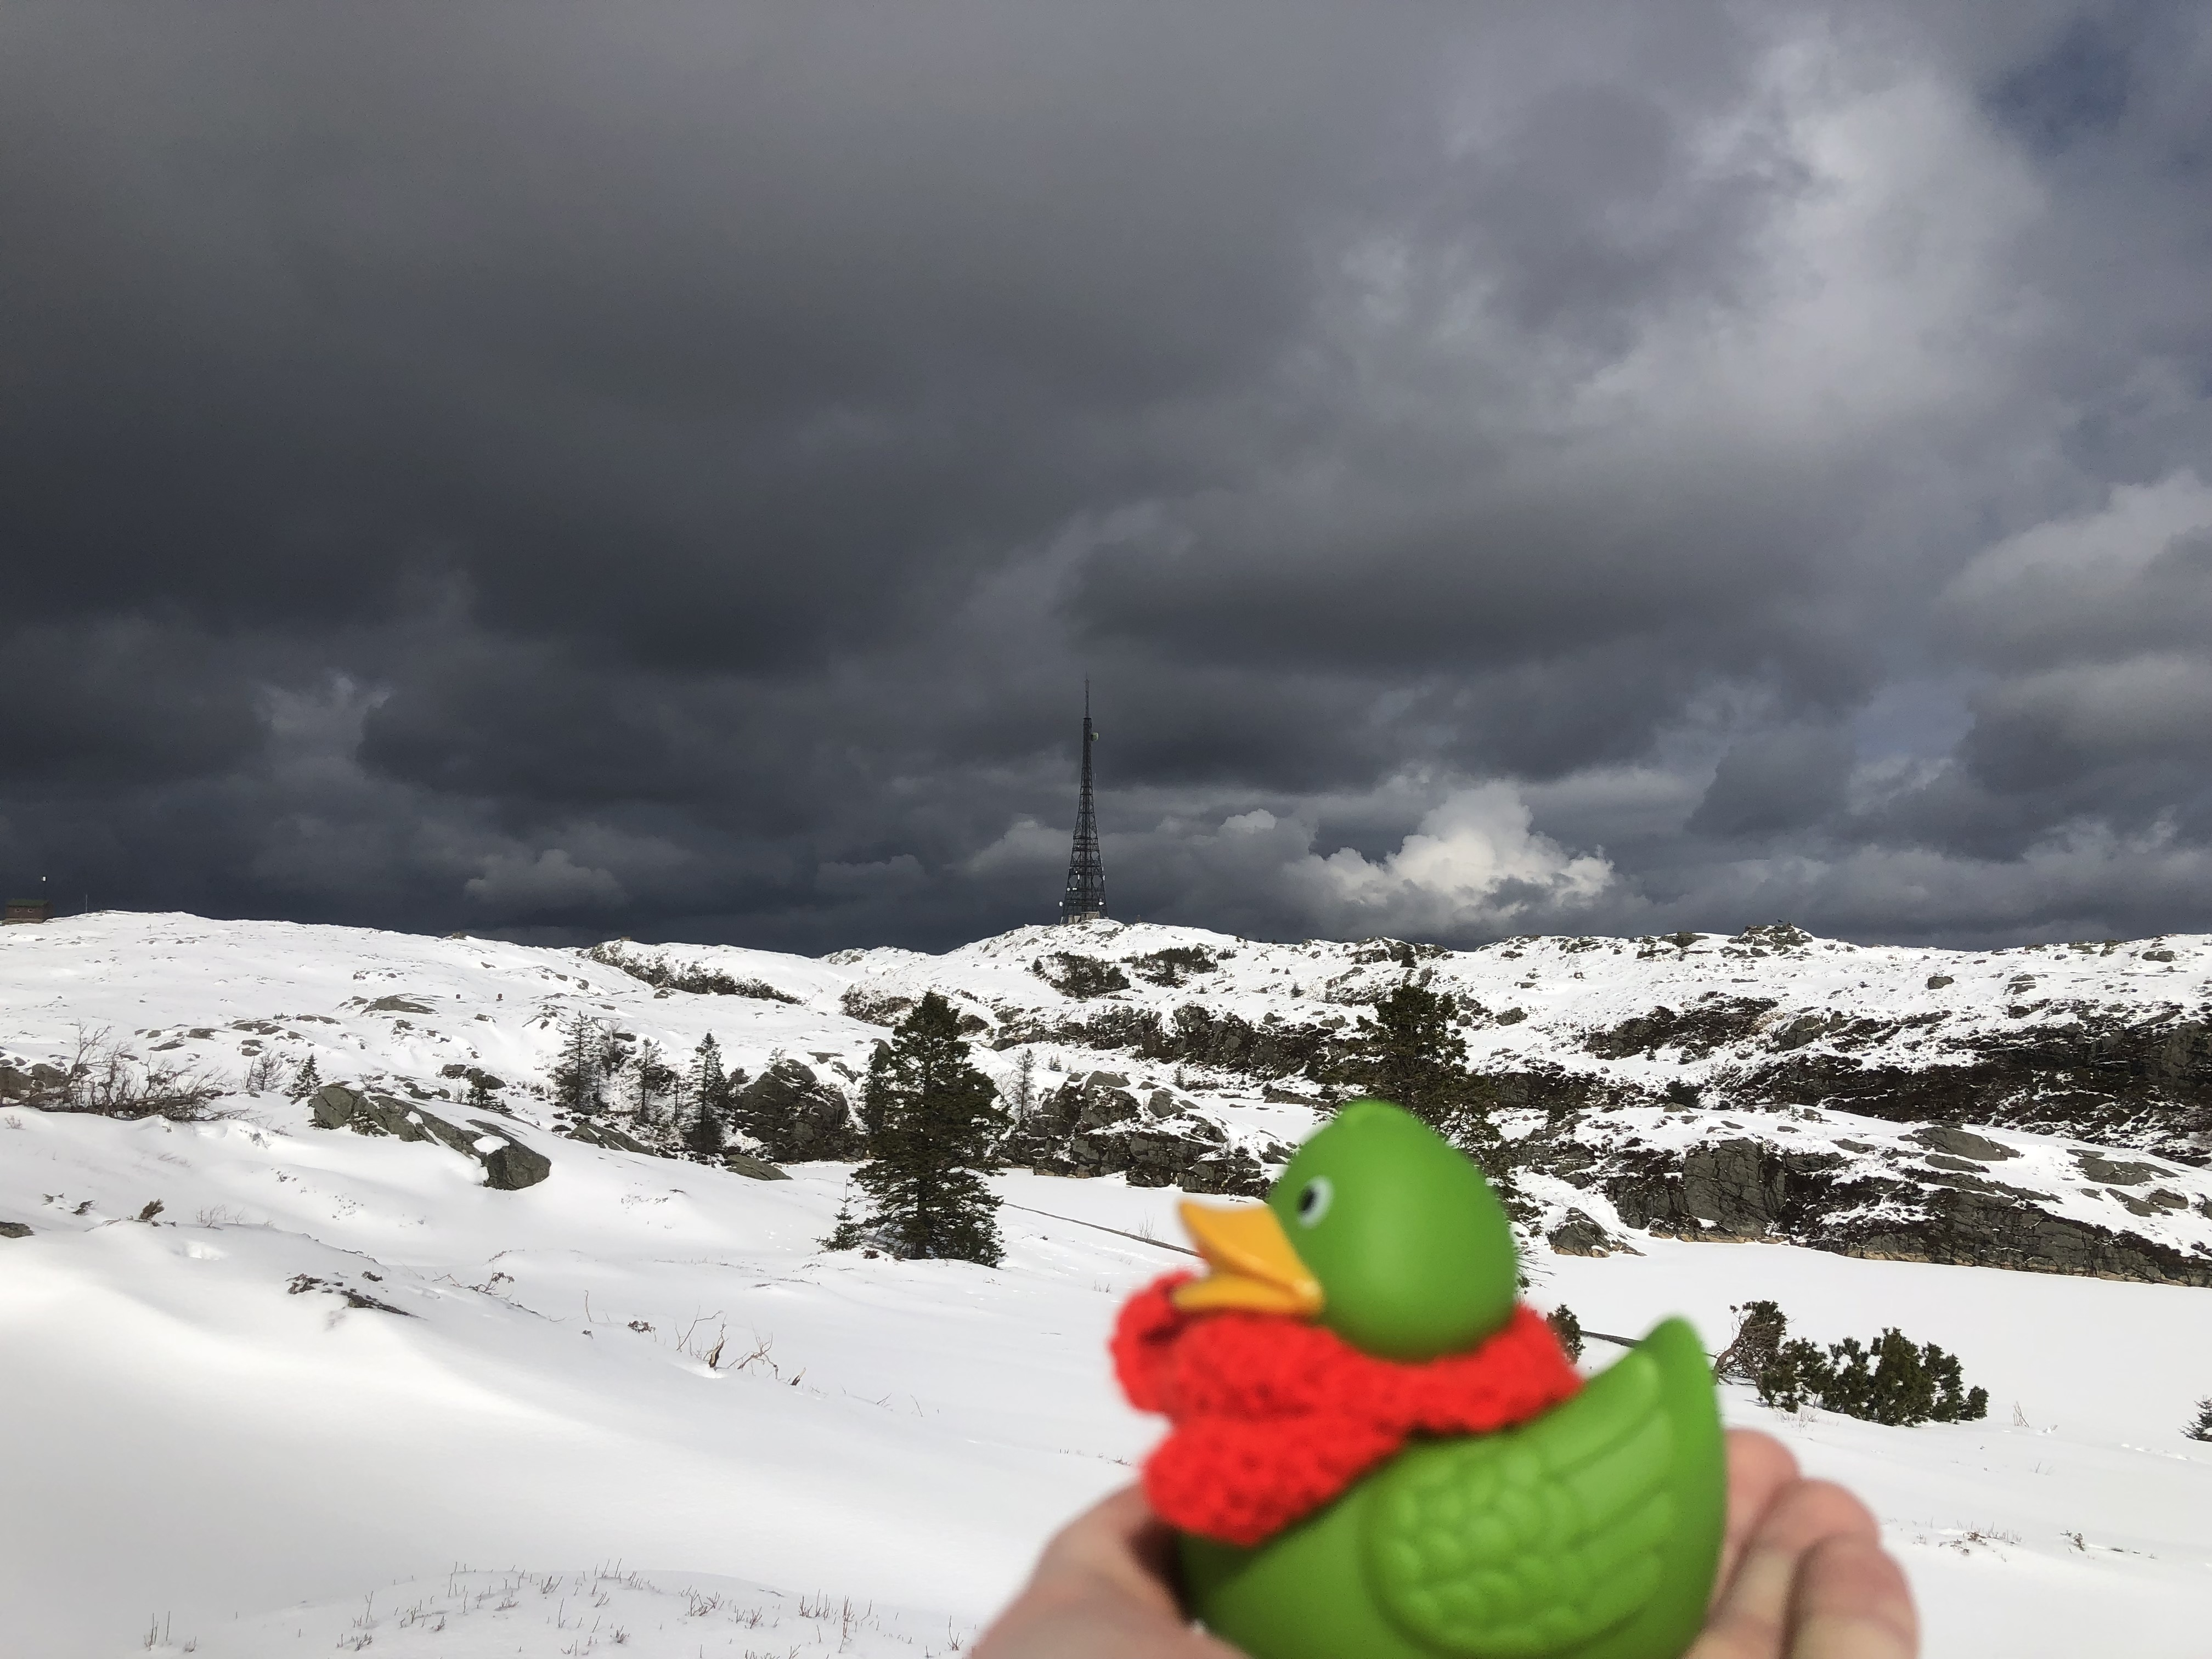
\includegraphics[height = 4.9cm]{guillaume6.jpg}
    \end{figure}
\end{frame}